\documentclass[a4paper]{article}
\usepackage{cmap}
\usepackage[utf8]{inputenc}
\usepackage[T2A]{fontenc}
\usepackage[english,russian]{babel} 
\usepackage[left=15mm, top=15mm, right=15mm, bottom=42mm, nohead, nofoot]{geometry}
\usepackage{blindtext}  % рыба-текст
\usepackage{graphicx}  % изобржаения
\usepackage{float} % плавающие объекты
\usepackage{wrapfig}  % изобржаения
\usepackage{tikz} % графика
\usepackage{xcolor} % определение цветов
\usepackage{nicefrac} % красивые дроби
\usepackage{cancel} % сокращение
\usepackage{amsmath,amsfonts,amssymb} % математический пакет
\usepackage{hyperref}  % гиперссылки
\usepackage{fancybox,fancyhdr} % хедер и футер
\usepackage{listings} % код
\usepackage{accsupp}
\usepackage{caption}
\captionsetup[figure]{name=Рисунок}
\pagestyle{fancy}
\fancyhf{}
\fancyhead[L]{Лабораторная работа №2}
\fancyhead[R]{\textit{Свободное движение, устойчивость}}
\fancyfoot[C]{\thepage}
\headsep=8mm
\footskip=20mm

\definecolor{urlcolor}{HTML}{3454D1}
\definecolor{linkcolor}{HTML}{3454D1}
\hypersetup{pdfstartview=FitH, linkcolor=linkcolor, urlcolor=urlcolor, colorlinks=true}

\definecolor{strings}{rgb}{0,0.6,0}
\definecolor{comments}{rgb}{0,0.3,0}
\definecolor{numbers}{rgb}{0.5,0.5,0.5}
\definecolor{keywords}{rgb}{0.09,0.61,0.95}
\definecolor{background}{rgb}{0.97,0.97,0.97}
\newcommand{\noncopynumber}[1]{%
    \BeginAccSupp{method=escape,ActualText={}}%
    #1%
    \EndAccSupp{}%
}
\lstdefinestyle{codestyle}{
    backgroundcolor=\color{background},
    commentstyle=\color{comments},
    keywordstyle=\color{keywords},
    stringstyle=\color{strings},
    numberstyle=\tiny\color{numbers}\noncopynumber,
    basicstyle=\ttfamily\footnotesize,
    breakatwhitespace=false,
    breaklines=true,
    captionpos=b,
    inputencoding=utf8,
    keepspaces=true,
    numbers=left,
    numbersep=5pt,
    showspaces=false,
    showstringspaces=false,
    showtabs=false,
    tabsize=2,
    extendedchars=true,
    literate=
    {а}{{\cyra}}1
    {б}{{\cyrb}}1
    {в}{{\cyrv}}1
    {г}{{\cyrg}}1
    {д}{{\cyrd}}1
    {е}{{\cyre}}1
    {ж}{{\cyrzh}}1
    {з}{{\cyrz}}1
    {и}{{\cyri}}1
    {й}{{\cyrishrt}}1
    {к}{{\cyrk}}1
    {л}{{\cyrl}}1
    {м}{{\cyrm}}1
    {н}{{\cyrn}}1
    {о}{{\cyro}}1
    {п}{{\cyrp}}1
    {р}{{\cyrr}}1
    {с}{{\cyrs}}1
    {т}{{\cyrt}}1
    {у}{{\cyru}}1
    {ф}{{\cyrf}}1
    {х}{{\cyrh}}1
    {ц}{{\cyrc}}1
    {ч}{{\cyrch}}1
    {ш}{{\cyrsh}}1
    {щ}{{\cyrshch}}1
    {ъ}{{\cyrhrdsn}}1
    {ы}{{\cyrery}}1
    {ь}{{\cyrsftsn}}1
    {э}{{\cyrerev}}1
    {ю}{{\cyryu}}1
    {я}{{\cyrya}}1
    {А}{{\CYRA}}1
    {Б}{{\CYRB}}1
    {В}{{\CYRV}}1
    {Г}{{\CYRG}}1
    {Д}{{\CYR96}}1
    {Е}{{\CYRE}}1
    {Ж}{{\CYRZH}}1
    {З}{{\CYRZ}}1
    {И}{{\CYRI}}1
    {Й}{{\CYRISHRT}}1
    {К}{{\CYRK}}1
    {Л}{{\CYRL}}1
    {М}{{\CYRM}}1
    {Н}{{\CYRN}}1
    {О}{{\CYRO}}1
    {П}{{\CYRP}}1
    {Р}{{\CYRR}}1
    {С}{{\CYRS}}1
    {Т}{{\CYRT}}1
    {У}{{\CYRU}}1
    {Ф}{{\CYRF}}1
    {Х}{{\CYRH}}1
    {Ц}{{\CYRC}}1
    {Ч}{{\CYRCH}}1
    {Ш}{{\CYRSH}}1
    {Щ}{{\CYRSHCH}}1
    {Ъ}{{\CYRHRDSN}}1
    {Ы}{{\CYRERY}}1
    {Ь}{{\CYRSFTSN}}1
    {Э}{{\CYREREV}}1
    {Ю}{{\CYRYU}}1
    {Я}{{\CYRYA}}1
}

\lstset{style=codestyle}

\addto\captionsrussian{
  \renewcommand{\contentsname}
    {\centering Содержание}
}


\newlength{\tempheight}
\newcommand{\Let}{
\mathbin{\text{\settoheight{\tempheight}{\mathstrut}\raisebox{0.4\pgflinewidth}{
\tikz[baseline=0.5ex,line cap=round,line join=round] \draw (0,0) --++ (0.3em,0) --++ (0,2.3ex) --++ (-0.3em,0);
}}}}
\newcommand*\squared[1]{\tikz[baseline=(char.base)]{
            \node[shape=rectangle,draw,inner sep=4pt] (char) {#1};}}
\newcommand*\msquared[1]{\tikz[baseline=(char.base)]{
            \node[shape=rectangle,draw,inner sep=4pt] (char) {$\displaystyle #1$};}}
\newcommand{\at}{\biggr\rvert}
\newcommand{\shiftright}[3]{\makebox[#2][r]{\makebox[#1][l]{#3}}}
\newcommand{\e}{\;\text{e}}
\let\oldint\int
\def\int{\oldint\limits}
\DeclareRobustCommand{\divby}{%
  \mathrel{\vbox{\baselineskip.65ex\lineskiplimit0pt\hbox{.}\hbox{.}\hbox{.}}}%
}

\newcommand\NB{\textbf{N\kern-0.32em\textcolor{red}{B}}}

\begin{document}

\begin{titlepage}
    \begin{center}
        Федеральное государственное автономное образовательное \\ учреждение высшего образования \\[6pt]
        САНКТ-ПЕТЕРБУРГСКИЙ НАЦИОНАЛЬНЫЙ \\ ИССЛЕДОВАТЕЛЬСКИЙ УНИВЕРСИТЕТ ИТМО \\[16pt]
        Факультет систем управления и робототехники \\[26em]
        Лабораторная работа №2\\[0.5em]
        \textbf{СВОБОДНОЕ ДВИЖЕНИЕ, УСТОЙЧИВОСТЬ}
    \end{center}\,\\[10em]
    \begin{flushright}
        Студент: Заводин Е.Ю.\\
        Лин САУ R23 бак 1.1.1 \\[0.5em]
        Преподаватели: Перегудин А.А.\\
        Пашенко А.В.
    \end{flushright}\,\\[6em]
    \begin{center}
        {\small Санкт-Петербург \\ 2025}
    \end{center}
\end{titlepage}
\setcounter{page}{2}
\tableofcontents\newpage

\section{Свободное движение}\

В задании рассматриваю систему 2-го порядка, заданную уравнением 

$$
\ddot{y}+a_1\dot{y} + a_0=a_0 u
$$\

Для этой системы составил структурную схему:

\begin{figure}[H]
    \centering
    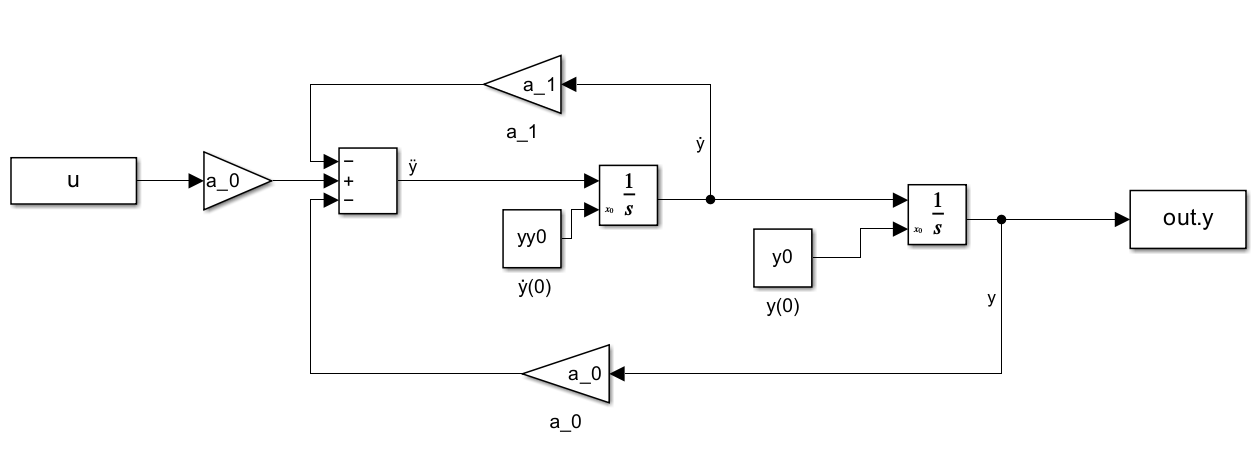
\includegraphics[width=0.75\linewidth]{ex1/scheme.png}
    \caption{Структурная схема системы из первого задания}
\end{figure}\ 

Для нахождения коэффициентов $a_0, a_1$ по заданным корням характеристического уравнения рассмотрим однородное дифференциальное уравнение для данной системы и его характеристическое:

$$
\ddot{y}+a_1\dot{y}+a_0=0,
$$
$$
\lambda^2+a_1\lambda+a_0=0.
$$\ 

Это уравнение представимо в виде $(\lambda-\lambda_1)(\lambda-\lambda_2)=0$, где $\lambda_1, \lambda_2$ -- корни уравнения. Раскрывая произведение, получим $\lambda^2 - (\lambda_1+ \lambda_2)\lambda + \lambda_1 \lambda_2=0$. Тогда

$$\lambda^2+a_1\lambda+a_0=\lambda^2 - (\lambda_1+ \lambda_2)\lambda + \lambda_1 \lambda_2=0.$$\ 

Сравнивая коэффициенты при одинаковых степенях $\lambda$, получим формулы для $a_1$ и $a_0$:

$$
a_1=-(\lambda_1+\lambda_2), a_0 = \lambda_1\lambda_2.
$$\

Формулы применимы и для действительных чисел, и для комплексно-сопряжённых, однако в комплексном случае ($\lambda_i=\alpha_i+\beta_i i$) вычислять буду следующим образом:

$$
a_1 = -(\alpha + \beta + \alpha-\beta) = -2\alpha, a_0 = (\alpha+\beta i)(\alpha -\beta i) = (\alpha^2-(\beta i)^2) =\alpha^2+\beta^2.
$$\

Для первого набора значений $\lambda_1 = \lambda_2 = -2.5$:

$$
a_0 = -2.5 \cdot (-2.5) = 6.25
$$
$$
a_1 = -(-2.5 + (-2.5)) = 5.
$$\


Свободная составляющая движения $y_{\text{св}}(t)$ для конкретного эксперимента может быть найдена суммированием мод, соответствующих корням характеристического уравнения, а затем подстановкой начальных условий для нахождения значений постоянных коэффициентов $C_i$.\

Так как корни характеристического уравнения первого эксперимента вещественные и кратные, общее решение полученного однородного дифференциального уравнения $\ddot{y} + 5 \dot{y} + 6.25y = 0$ будет выглядеть следующим образом:

$$
y(t) = C_1e^{-2.5t} + C_2te^{-2.5t}
$$\ 

Продифференцируем получившееся уравнение по $t$:

$$
\dot{y}(t) = (C_1e^{-2.5t}+C_2te^{-2.5t})'_t = -2.5C_1e^{-2.5t}+C_2(e^{-2.5t}-2.5te^{-2.5t}) = e^{-2.5t}(-2.5C_1 + C_2-2.5C_2t).
$$\

Коэффициенты $C_1, C_2$ найдём из начальных условий $y(0) = 1, \dot{y}(0) = 0$:

$$
y(0) = 1 \Rightarrow C_1e^{-2.5 \cdot 0} + C_2 \cdot0 \cdot e^{-2.5 \cdot 0} = 1 \Rightarrow C_1 = 1
$$
$$
\dot{y}(0) = 0 \Rightarrow e^{-2.5\cdot 0}(-2.5C_1 + C_2-2.5C_2\cdot 0)= -2.5C_1 + C_2=0 \Rightarrow C_2 = 2.5
$$\ 

Получившееся аналитическое выражение для свободной составляющей движения системы:

$$y_{\text{св}}(t) = e^{-2.5t} + 2.5te^{-2.5t}$$\

Расчёты для остальных экспериментов выполнены аналогично и внесены в таблицу.\
\renewcommand{\arraystretch}{1.5}
\begin{table}[H]
    \centering
    \begin{tabular}{|c|c|c|c|}
      \hline
      \multicolumn{2}{|c|}{Входные значения} & \multicolumn{2}{|c|}{Результаты вычисления} \\
      \hline
      $\lambda_1, \lambda_0$ & $y(0), \dot{y}(0)$ & $
      a_1, a_0$ & $y_{\text{св}}(t)$ \\
      \hline
      $-2.5, -2.5$ & $1, 0$ & 5, 6.25 & $e^{-2.5t} + 2.5te^{-2.5t}$ \\
      \hline
      $-1 \pm 8i$ & $1, 0$ & 2, 65 & $0.125\sin\left(8\,t\right)e^{-t}+\cos\left(8\,t\right)e^{-t}$ \\
      \hline
      $\pm 8i$ & $1, 0$ & 0, 64 & $\cos\left(8\,t\right)$ \\
      \hline
      $1 \pm 8i$ & $0.05, 0$ & -2, 65 & $\frac{1}{20}{e}^{t}\cos\left(8\,t\right)-\frac{1}{160}{e}^{t}\,\sin\left(8\,t\right)$ \\
      \hline
      $2.5, 2.5$ & $0.05, 0$ & -5, 6.25 & $\frac{1}{20}{e}^{\frac{5\,t}{2}}-\frac{t}{8}{e}^{\frac{5\,t}{2}}\,$ \\
      \hline
      $-0.6, 0.6$ & $0, 0.1$ & 0, -0.36 & $\frac{1}{12}{e}^{0.6t}-\frac{1}{12}\,{e}^{-0.6t}$ \\
      \hline
    \end{tabular}
    \caption{Исходные данные и результаты вычислений для задания 1}
\end{table}

Аналитические выражения для каждого из экспериментов найдены, теперь можно проверить вычисления сравнением с моделированием соответствующей структурной схемы без входного воздействия $(u(t) = 0)$, подставляя вычисленные коэффициенты дифференциального уравнения и экспериментальные данные для начальных условий:

\begin{figure}[H]
    \begin{minipage}{0.5\textwidth}
        \centering 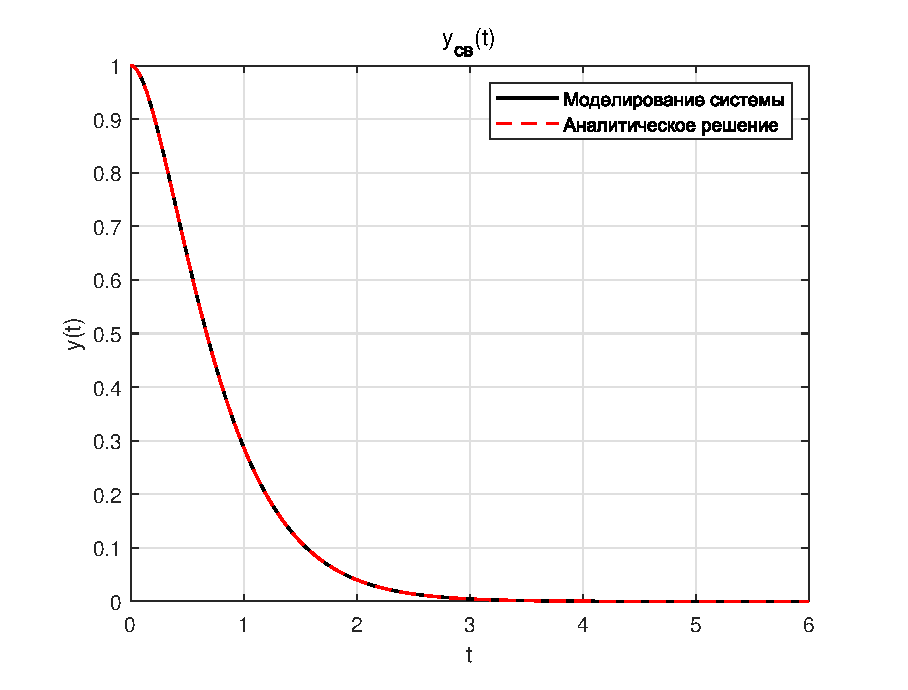
\includegraphics[width=\textwidth]{ex1/1.eps}
        \caption{Выход $y_{\text{св}}(t)$ для системы 1,}
        \centerline{$a_0 = 6.25, a_1 = 5, y(0) = 1, \dot{y}(0) = 0$}
    \end{minipage}\hfill
    \begin{minipage}{0.5\textwidth}
        \centering 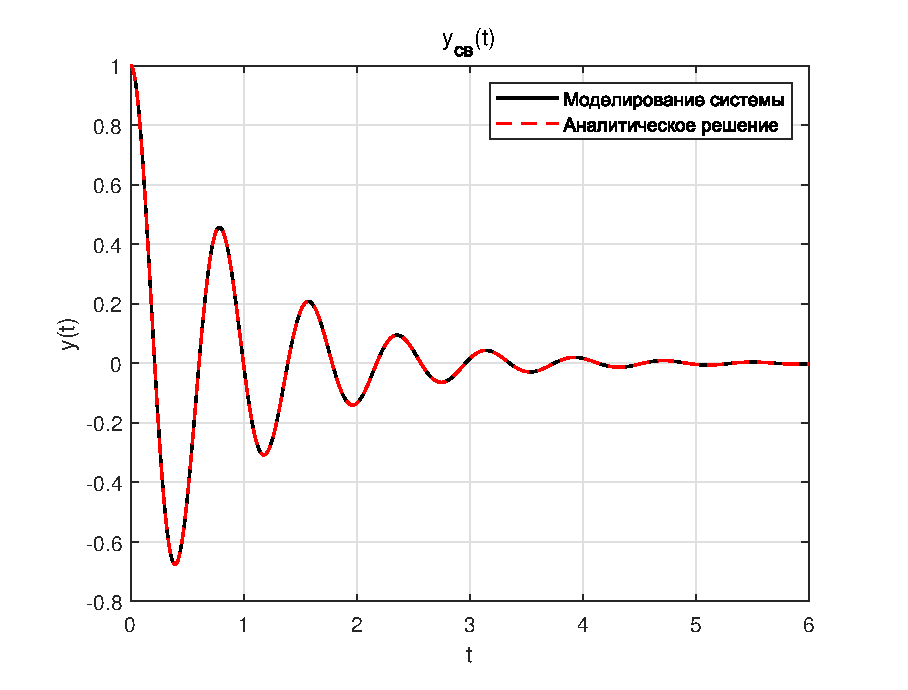
\includegraphics[width=\textwidth]{ex1/2.eps}
        \caption{Выход $y_{\text{св}}(t)$ для системы 2,}
        \centerline{$a_0 = 65, a_1 = 2, y(0) = 1, \dot{y}(0) = 0$}
    \end{minipage}\\[1em]
\end{figure}\noindent\

Судя по графику, первая система асимптотически устойчива, это наблюдение подтверждается корневым критерием. Корни $\lambda_1 = \lambda_2 = -2.5$ действительные, соответствующие им моды стремятся к 0 при $t \to \infty$.\ 

Вторая система также асимптотически устойчива и по графику выхода, и по корневому критерию ($\lambda_{1,2} = -1\pm 8i \Rightarrow \text{Re}(\lambda_{1,2})=-1$). Видны затухающие колебания, вызванные наличием гармонических компонент в решении этой системы.

\begin{figure}[H]
    \begin{minipage}{0.5\textwidth}
        \centering 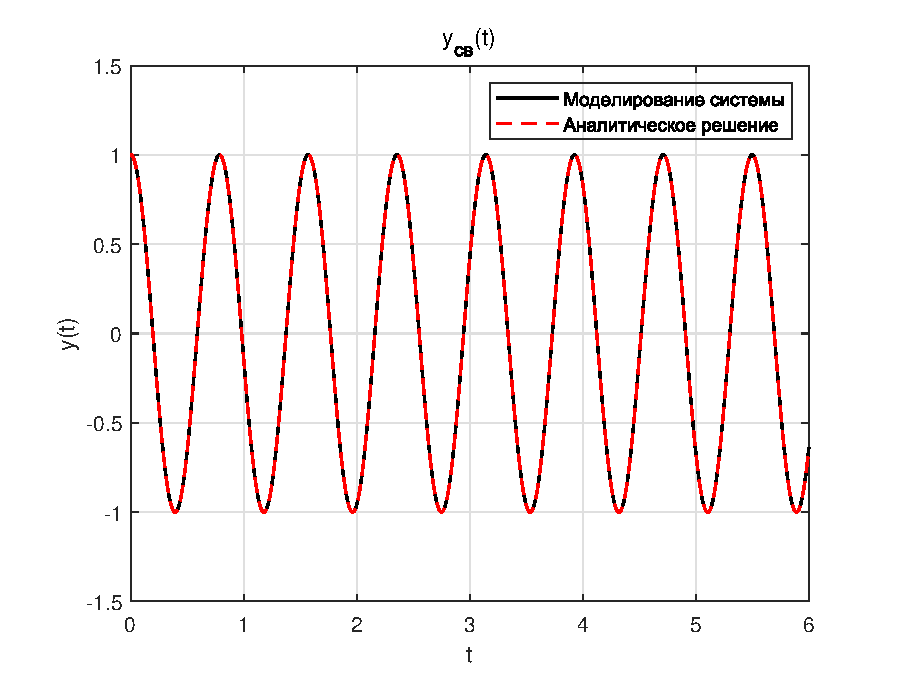
\includegraphics[width=\textwidth]{ex1/3.eps}
        \caption{Выход $y_{\text{св}}(t)$ для системы 3,}
        \centerline{$a_0 = 64, a_1 = 0, y(0) = 1, \dot{y}(0) = 0$}
    \end{minipage}\hfill
    \begin{minipage}{0.5\textwidth}
        \centering 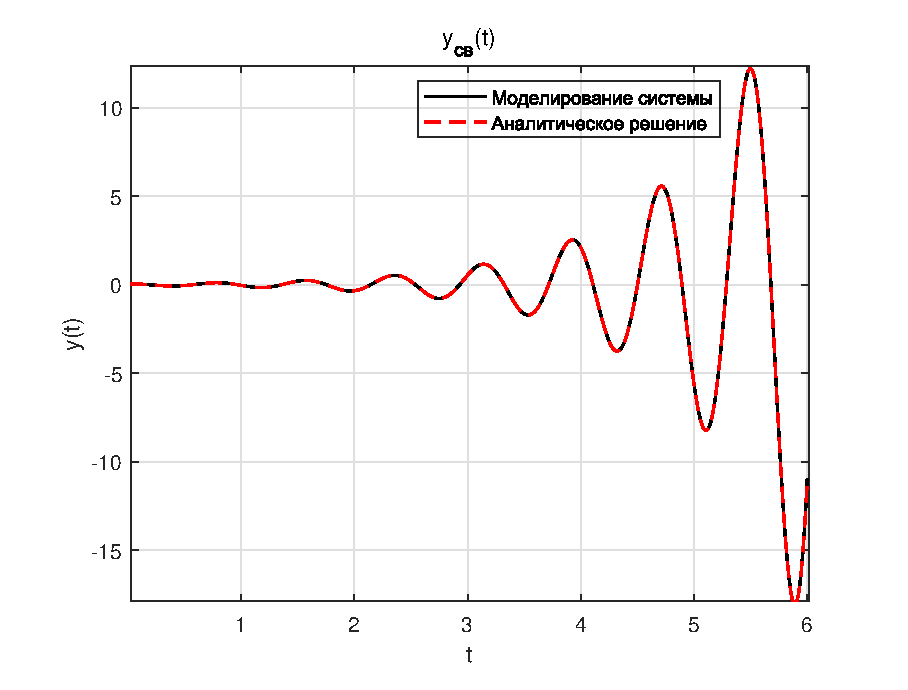
\includegraphics[width=\textwidth]{ex1/4.eps}
        \caption{Выход $y_{\text{св}}(t)$ для системы 4,}
        \centerline{$a_0 = 65, a_1 = -2, y(0) = 0.05, \dot{y}(0) = 0$}
    \end{minipage}\\[1em]
\end{figure}\noindent\

В случае третьей системы появляются колебания, которые не затухают при $t \to \infty$, значит, система устойчива, но не асимптотически -- устойчива по Ляпунову. Это же подтверждает и анализ по корневому критерию -- действительная часть $\lambda_{1,2} = \pm 8i$ равна 0.\ 

Четвертая система демонстрирует ситуацию, прямо противоположную второму случаю -- система со временем расходится, гармонические колебания нарастают, система неустойчива. Это же подтверждает и корневой анализ, $\lambda_{1,2} = 1\pm8i$, следовательно, полюса системы на комплексной плоскости находятся справа от оси ординат.

\begin{figure}[H]
    \begin{minipage}{0.5\textwidth}
        \centering 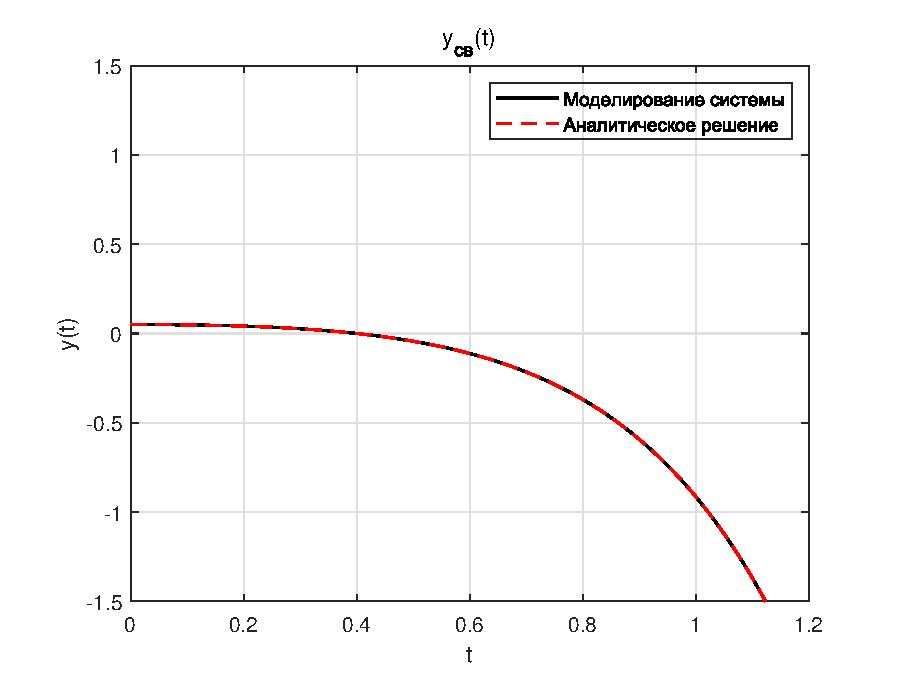
\includegraphics[width=\textwidth]{ex1/5.eps}
        \caption{Выход $y_{\text{св}}(t)$ для системы 5,}
        \centerline{$a_0 = 6.25, a_1 = -5, y(0) = 0.05, \dot{y}(0) = 0$}
    \end{minipage}\hfill
    \begin{minipage}{0.5\textwidth}
        \centering 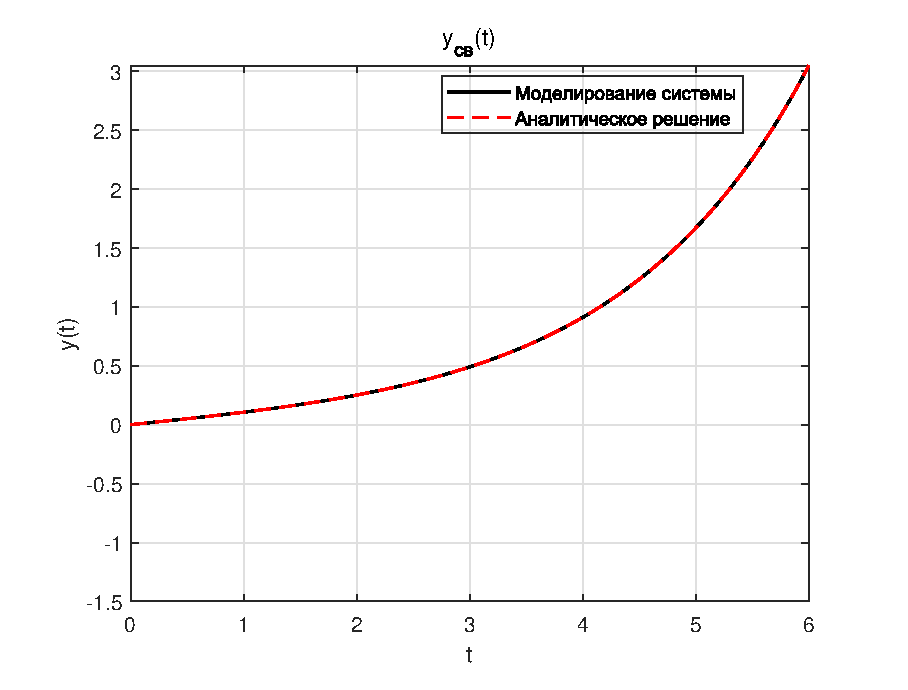
\includegraphics[width=\textwidth]{ex1/6.eps}
        \caption{Выход $y_{\text{св}}(t)$ для системы 6,}
        \centerline{$a_0 = -0.36, a_1 = 0, y(0) = 0, \dot{y}(0) = 0.1$}
    \end{minipage}\\[1em]
\end{figure}\noindent\

Пятая же система также неустойчива, но в этот раз без гармонической составляющей. $\lambda_{1,2} = 2.5$, что также указывает на неустойчивость системы.\ 

По графику выхода свободной составляющей движения шестой системы на лицо неустойчивость, корни системы $(\lambda_1 = 0.6, \lambda_2 = -0.6)$ равны по модулю и противоположны по знаку, один из них больше ноля, что и приводит к неустойчивости -- соответствующая ему мода является растущей экспонентой.

\subsection{Выводы}\

Моделирование во всех случаях совпало с аналитическими расчётами, что говорит о том, что ошибок при нахождении выражений для свободных составляющих движения допущено не было. Проанализирована устойчивость полученных систем, результаты анализа устойчивости по корневому критерию соответствуют графикам.

\section{Область устойчивости}\

В задании рассматривается следующая структурная схема:

\begin{figure}[H]
    \centering
    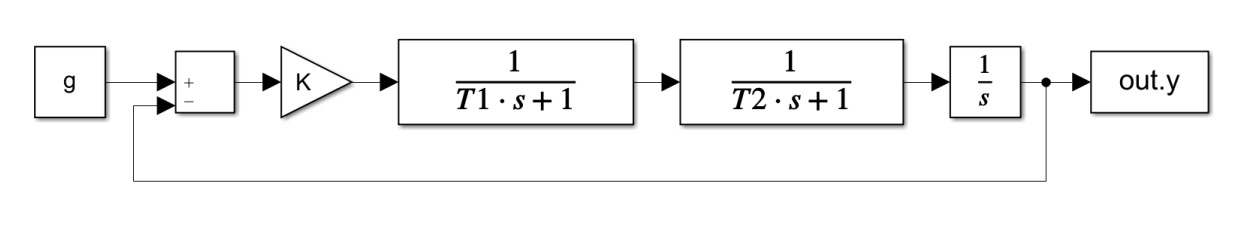
\includegraphics[width=0.75\linewidth]{ex2/scheme.png}
    \caption{Схема моделирования для задания 2}
\end{figure}\ 

Рассмотрим передаточные функции $\frac{1}{T_1 \cdot s + 1}$ и $\frac{1}{T_2\cdot s + 1}$, для которых по заданию предполагается определить такие постоянные времени $T_1, T_2$, при которых полюса передаточных функций равняются $\lambda_1 = \lambda_2 = -2.5$.\ 

Полюс первой ПФ $\frac{1}{T_1 \cdot s + 1}$ находится в точке $T_1\cdot s = -1$. Подставляя $s = -2.5$, получаем $-2.5 = -\frac{1}{T_1} \Rightarrow T_1 = 0.4$. Так как вторая передаточная функция отличается от первой только постоянной времени, то для неё аналогично $T_2 = T_1 = 0.4$.\ 

Структурная схема, рассматриваемая в задании, является замкнутой схемой с отрицательной обратной связью, а значит, уравнение в операторной форме, соответствующее этой схеме, будет выглядеть следующим образом:

$$
Y(s)=W(s)(G(s)-Y(s)),
$$
где $W(s) = \frac{K}{(T_1s+1)(T_2s+1)s}$.\

Сведём это выражение к конкретному дифференциальному уравнению.

$$
Y(s)=W(s)(G(s)-Y(s)) \Leftrightarrow [1+W(s)]Y(s)=W(s)G(s)
$$\

Подставляя $W(s)$ и домножая на его знаменатель, получаем:

$$
[1+W(s)]Y(s)=W(s)G(s) \Leftrightarrow \left[1 + \frac{K}{(T_1s+1)(T_2s+1)s}\right]Y(s)=\frac{K}{(T_1s+1)(T_2s+2)s}G(s) \Leftrightarrow
$$

$$
\left((T_1s+1)(T_2s+1)s + K\right)Y(s)=KG(s).
$$\

Раскрыв скобки и перейдя от операторной формы, получим:

$$
\left((T_1s+1)(T_2s+1)s + K\right)Y(s) = ((T_1T_2s^2+T_1s+T_2s+1)s + K)Y(s) =
$$

$$
= (T_1T_2s^3+T_1s^2+T_2s^2+s+K)Y(s) = T_1T_2\dddot{y} + (T_1 + T_2)\ddot{y} + \dot{y} + Ky.
$$\ 

Рассмотрим однородное уравнение, и для исследования на устойчивость при помощи использования следствия из критерия Гурвица поделим уравнение на коэффициент перед $\dddot{y}$:

$$
T_1T_2\dddot{y} + (T_1 + T_2)\ddot{y} + \dot{y} + Ky = \dddot{y}+\frac{T_1+T_2}{T_1T_2}\ddot{y} + \frac{1}{T_1T_2}\dot{y}+\frac{K}{T_1T_2}y = 0
$$\ 

Следствие из критерия Гурвица для дифференциального уравнения третьего порядка вида $\dddot{y}+a_2\ddot{y}+a_1\dot{y}+a_0y=0$ гласит, что система асимптотически устойчива тогда и только тогда, когда $a_2, a_1, a_0 > 0$ и $a_2a_1>a_0$. Проверим, при каких $K, T_2$ это выполняется для нашего уравнения при фиксированном найденном ранее значении $T_1 = 0.4$:

$$
\dddot{y}+\frac{0.4+T_2}{0.4T_2}\ddot{y} + \frac{1}{0.4T_2}\dot{y}+\frac{K}{0.4T_2}y = 0 \Rightarrow a_2 = \frac{0.4+T_2}{0.4T_2}, a_1 = \frac{1}{0.4T_2}, a_0 = \frac{K}{0.4T_2}.
$$\ 

Составим систему из уравнений, которые обеспечат асимптотическую устойчивость:

$$
\begin{cases}
    \frac{0.4 + T_2}{0.4T_2}>0 \\
    \frac{1}{0.4T_2}>0 \\
    \frac{K}{0.4T_2}>0\\
    \frac{0.4+T_2}{0.4T_2}\cdot\frac{1}{0.4T_2}>\frac{K}{0.4T_2}
\end{cases}
$$\ 

Случай $T_2<0$ можем не рассматривать, так как при нём не будет выполняться второе неравенство. Также не берём в расчёт вариант $T_2 = 0$, так как при нём возникает деление на 0. Тогда, при $T_2 > 0$, система сводится к следующей:

$$
\begin{cases}
    T_2>-0.4 \\
    K>0\\
    \frac{0.4+T_2}{0.4T_2}>K \Leftrightarrow K<\frac{0.4+T_2}{0.4T_2}
\end{cases}
$$\

В итоге получаем, что система находится на границе устойчивости при $K(T_2) = \frac{0.4+T_2}{0.4T_2}$\ 

Так как фиксированное рассчитанное ранее значение $T_2$ совпадает с $T_1$, то в пространстве параметров $K, T_1$ граница устойчивости $K(T_1)$ будет выглядеть так же, как и $K(T_2)$: $K(T_1) = \frac{0.4+T_1}{0.4T_1}$.\ 

\begin{figure}
    \centering
    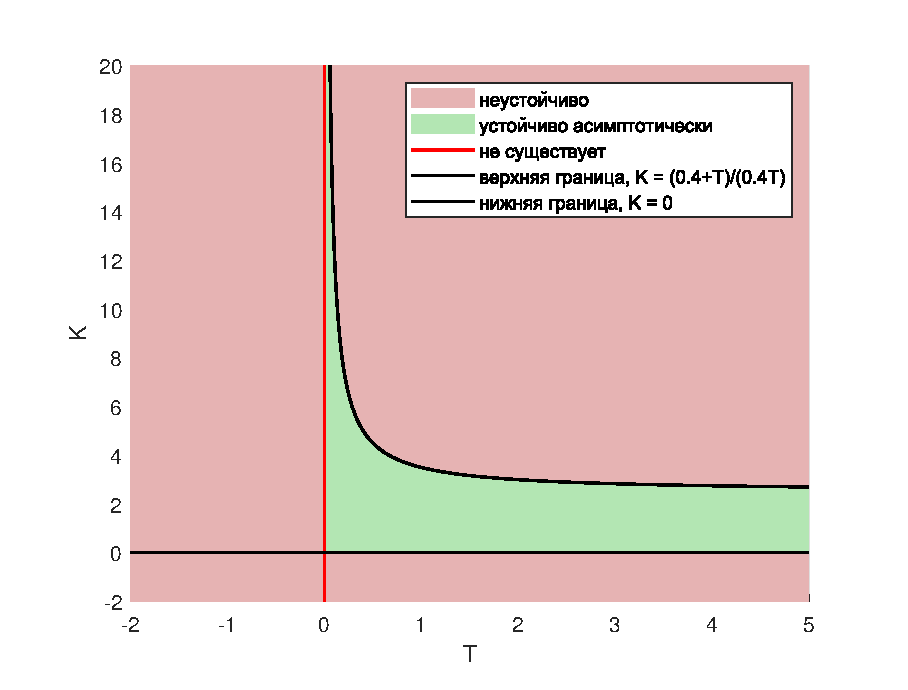
\includegraphics[width=0.75\linewidth]{ex2/border.eps}
    \caption{Графическое изображение границы устойчивости системы}
\end{figure}\

При наборе $K = 3.5, T_2 = 1, T_1 = 0.4$ система находится на границе устойчивости, при $K = 10, T_2 = 1, T_1 = 0.4$ система неустойчива, а при $K = 0.5, T_2 = 1, T_1 = 0.4$ -- асимптотически устойчива. Промоделируем указанные наборы параметров, чтобы убедиться в этом:

\begin{figure}[H]
    \centering
    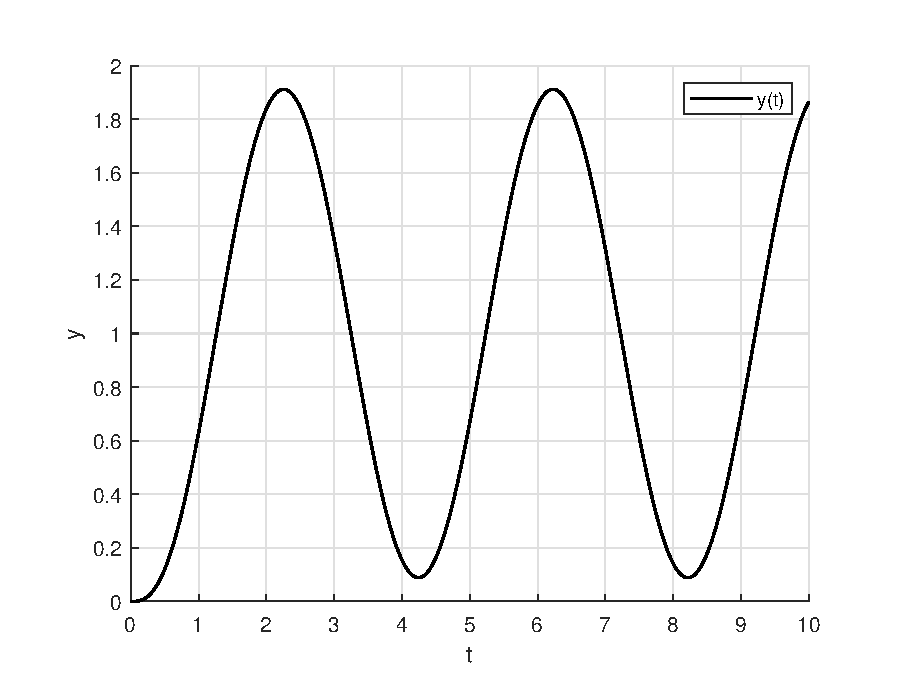
\includegraphics[width=0.75\linewidth]{ex2/3.5.eps}
    \caption{$K = 3.5, T_2 = 1, T_1 = 0.4$}
\end{figure}\

На данном графике траектория $y(t)$ ограничена, при $t \to \infty$ она не сойдётся к начальному воздействию, но и не уйдёт в бесконечность. Система устойчива, но не асимптотически -- на границе устойчивости.

\begin{figure}[H]
    \centering
    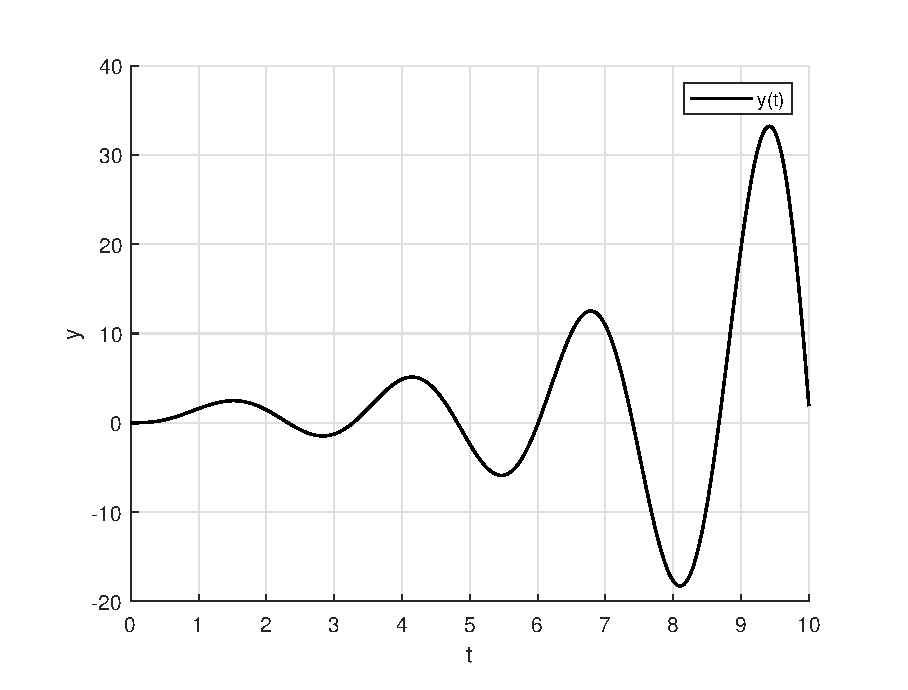
\includegraphics[width=0.75\linewidth]{ex2/10.eps}
    \caption{$K = 10, T_2 = 1, T_1 = 0.4$}
\end{figure}\

График расходящийся, система неустойчива.

\begin{figure}[H]
    \centering
    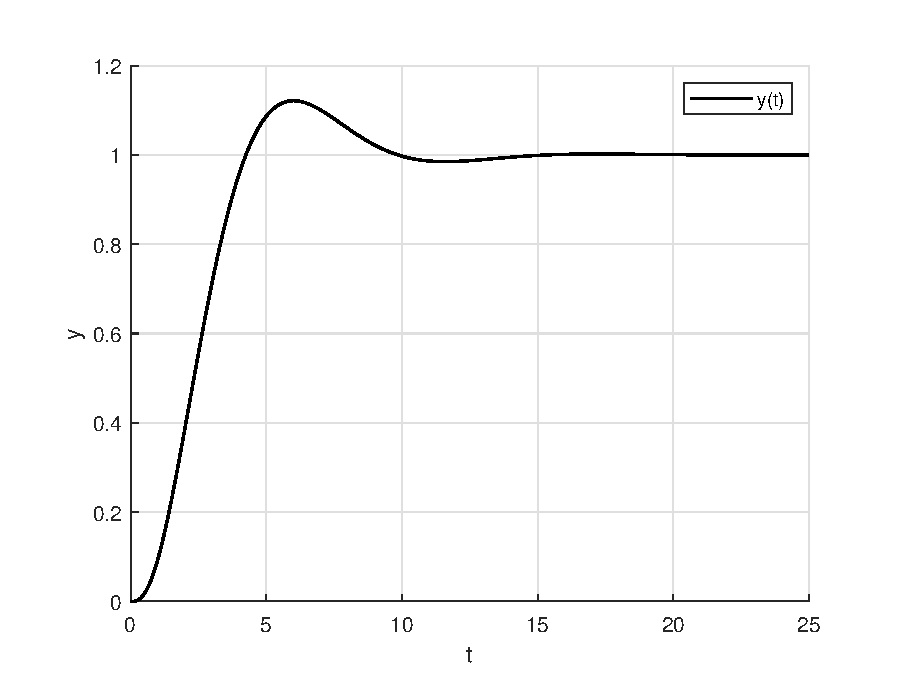
\includegraphics[width=0.75\linewidth]{ex2/0.5.eps}
    \caption{$K = 0.5, T_2 = 1, T_1 = 0.4$}
\end{figure}\

Можно заметить, что график сходится к внешнему воздействию $u(t) = 1$, и $y(t) \to 1$ при $t \to \infty$, а значит, система асимптотически устойчива.

\subsection{Выводы}\

Устойчивость системы, представленной в виде линейного дифференциального уравнения, определяется коэффициентами перед зависимыми переменными и их производными, она может быть определена заранее без решения самого уравнения при помощи критерия Гурвица и следствий из него.

\section{Автономный генератор}\

Рассмотрим систему вида 

$$
\begin{cases}
    \dot{x} = Ax \\
    g = Cx,
\end{cases} \ \ \ \ \ \ \ x(0).
$$\ 

Найдём такие $A, C, x(0)$, чтобы выход системы совпадал с выходом $g_{\text{ж}}(t) = \cos{5t} + e^{t} + e^{-5t}$. Для этого вспомним, что свободное движение в этом случае по аналогии с системами в форме В-В (только там моды вместо элементов матричной экспоненты) определяется формулой $y_{\text{св}} = C e^{At}x(0)$.\ 

Сперва рассчитаем элементы матрицы $A$. Это можно легко осуществить, вспомнив, как устроены жордановы матрицы -- они состоят из жордановых клеток, формируемых из собственных чисел матрицы. А собственные числа матрицы, в свою очередь, совпадают с корнями характеристического уравнения, соответствующего системе в матричном виде. То есть, для построения матрицы $A$ из решения системы нужно выделить отдельные моды, затем понять, каким корням они соответствуют, затем принять эти корни за собственные числа матрицы $A$, и составить матрицу $A$ из жордановых клеток.\ 

Первым делом определим корни характеристического уравнения из выхода $g_{ж}(t) = \cos{5t} + e^{t} + e^{-5t}$. Моды $e^{t}$ и $e^{-5t}$ соответствуют корням $\lambda_1 = 1, \lambda_2 = -5$, а $\cos{5t}$ -- корням $\lambda_{1,2} = \pm 5i$. Комплексно-сопряжённые числа не существуют поодиночке в качестве корней характеристического уравнения, поэтому можно считать, что также имеется мода $0\sin{5t}$ в пару к $\cos{5t}$. Тогда можем составить $A$ из жордановых клеток:

$$
A = \begin{bmatrix}
    1 & 0 & 0 & 0 \\ 
    0 & -5 & 0 & 0 \\ 
    0 & 0 & 0 & 5 \\ 
    0 & 0 & -5 & 0
\end{bmatrix}
$$

$$
e^{At} = \begin{bmatrix}
    e^t & 0 & 0 & 0 \\ 
    0 & e^{-5t} & 0 & 0 \\ 
    0 & 0 & \cos{5t} & \sin{5t} \\ 
    0 & 0 & -\sin{5t} & \cos{5t}
\end{bmatrix}
$$

$$
e^{At}x(0) = \begin{bmatrix}
    e^t & 0 & 0 & 0 \\ 
    0 & e^{-5t} & 0 & 0 \\ 
    0 & 0 & \cos{5t} & \sin{5t} \\ 
    0 & 0 & -\sin{5t} & \cos{5t}
\end{bmatrix}\begin{bmatrix}
    a_1 \\ 
    a_2 \\ 
    a_3 \\ 
    a_4
\end{bmatrix} = \begin{bmatrix}
    a_1e^t\\
    a_2e^{-5t} \\ 
    a_3\cos{5t} + a_4\sin{5t} \\ 
    -a_3\sin{5t} + a_4\cos{5t}
\end{bmatrix}$$

$$
Ce^{At}x(0) = \begin{bmatrix}
    a_1e^t\\
    a_2e^{-5t} \\ 
    a_3\cos{5t} + a_4\sin{5t} \\ 
    -a_3\sin{5t} + a_4\cos{5t}
\end{bmatrix}\begin{bmatrix}
    c_1 & c_2 & c_3 & c_4
\end{bmatrix}=$$
$$=c_1a_1e^t + c_2a_2 e^{-5t}+c_3a_3\cos{5t} + c_4a_4\sin{5t}-c_3a_3\sin{5t}+c_4a_4\cos{5t}.
$$\ 

Сравним получившееся выражение с исходным выходом:

$$c_1a_1e^t + c_2a_2 e^{-5t}+c_3a_3\cos{5t} + c_4a_4\sin{5t}-c_3a_3\sin{5t}+c_4a_4\cos{5t} = \cos{5t} + e^{t} + e^{-5t}
$$\ 

Тогда для нахождения коэффициентов можем составить систему:

$$
\begin{cases}
    c_1a_1 = 1 \\
    c_2a_2 = 1 \\ 
    c_3a_3 + c_4a_4 = 1 \\
    c_4a_4 - c_3a_3 = 0
\end{cases}
$$\ 

У системы нет единого решения, можем взять любой подходящий набор коэффициентов. Пусть $c_1 = c_2 = a_1 = a_2 = 1, c_3 = 2, c_4 = 2, a_3 = 0.25, a_4 = 0.25$. Тогда $C$ и $x(0)$ выглядят так:

$$
C = \begin{bmatrix}
    1 & 1 & 2 & 2
\end{bmatrix}, x(0) = \begin{bmatrix}
    1 \\
    1 \\ 
    0.25 \\ 
    0.25
\end{bmatrix}.
$$\

Проверим правильность выбранных параметров моделированием и сравнением с исходным выражением:

\begin{figure}[H]
    \centering
    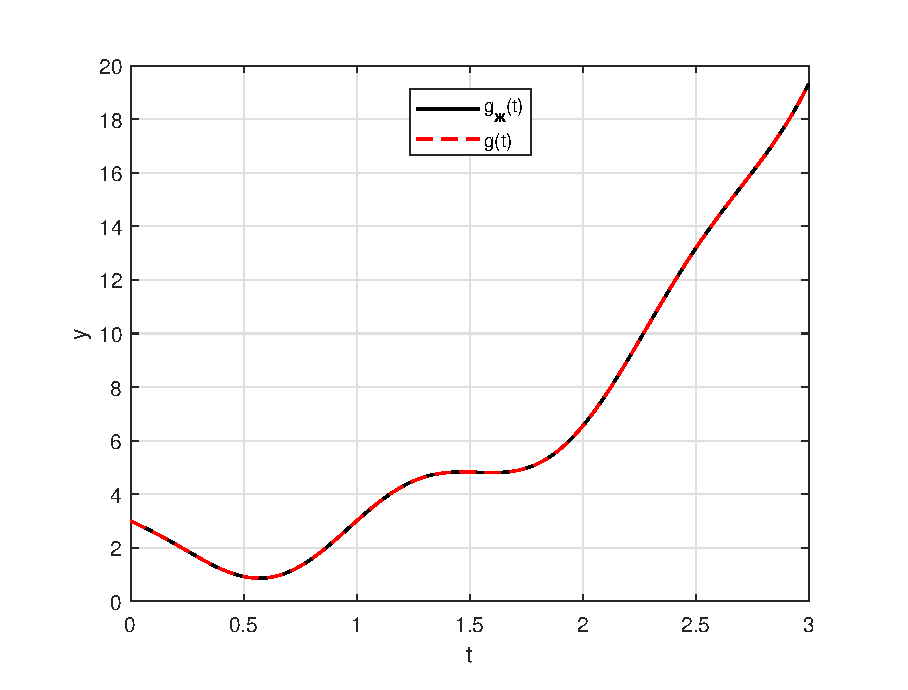
\includegraphics[width=0.65\linewidth]{ex3/compare.eps}
    \caption{Сравнение выхода системы, заданной формулой, и выхода генератора}
\end{figure}

\begin{figure}[H]
    \centering
    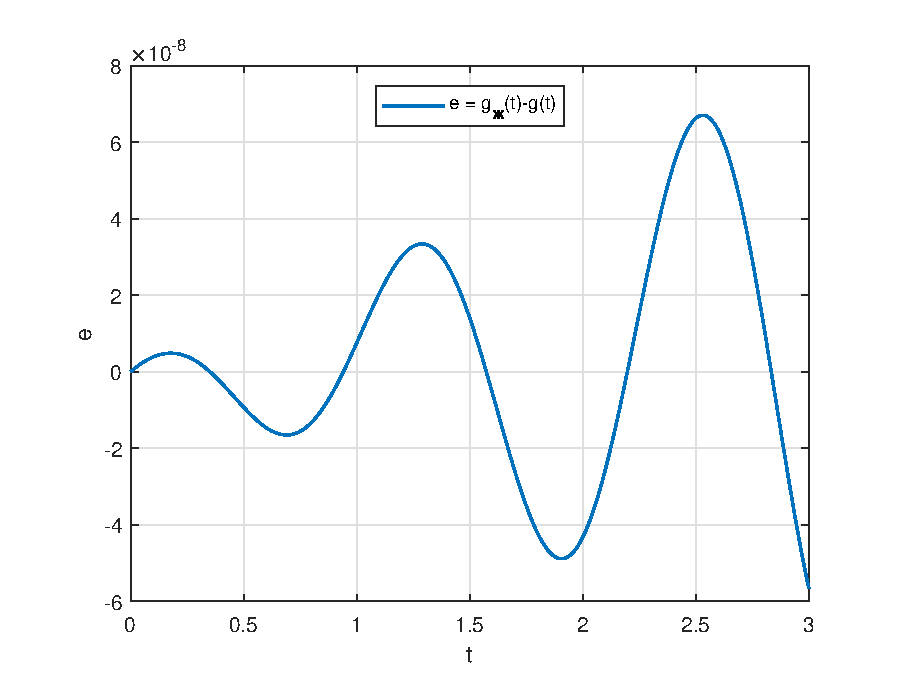
\includegraphics[width=0.65\linewidth]{ex3/error.eps}
    \caption{График ошибки в виде разницы полученных выходов}
\end{figure}\ 

По сравнительному графику выходов кажется, что графики идеально совпадают, однако график ошибки ясно даёт понять, что это не так -- со временем ошибка накапливается (её график расходится), и при $t \to \infty$ графики будут бесконечно далеки друг от друга, но при малых значениях $t$ ошибка незначительна.

\section{Вывод по работе}\ 

В ходе выполнения работы я ознакомился со свободным движением -- увидел, как системы ведут себя при отсутствии входного сигнала, в каких случаях они устойчивы, явным образом определил границу устойчивости для одной из систем, убедился в том, что по разные стороны этой границы система ведёт себя по-разному, также рассмотрел систему в формате В-С-В без входного воздействия (С-В?), ощутил связь между системой такого вида и системой, заданной дифференциальным уравнением, тот факт, что собственные числа матрицы системы это корни характеристического уравнения соответствующей системы в виде дифференциального уравнения, позволил выполнить третье задание. 

\newpage

\section{Приложение А. Код для выполнения заданий}

\subsection*{Листинг 1. Код для выполнения задания 1}

\begin{lstlisting}[caption={Код для построения графиков для задания 1}, language=matlab]
% clear all;
close all;
t = (0:0.001:6)';
a_0 = -0.36;
a_1 = 0;
y0 = 0;
yy0 = 0.1;

out = sim('ex1/model.slx','StopTime','6');
y_model = out.y;
y_t = figure;

y_model.plot('black', LineWidth=1.2)
grid on;
title('y_{св}(t)', 'Interpreter', 'tex', FontWeight='normal')
hold on;

% f = exp(-2.5.*t)+2.5.*t.*exp(-2.5.*t);
% f = 0.125.*sin(8.*t).*exp(-t) + cos(8.*t).*exp(-t);
% f = cos(8.*t);
% f = (1/20).*exp(t).*cos(8.*t)-(1/160).*exp(t).*sin(8.*t);
% f = (1/20 - t./8).*exp((2.5).*t);
f = (1/12).*exp(0.6.*t)-(1/12).*exp(-0.6.*t);
plot(t, f, '--red', LineWidth=1.2);
xlabel('t'), ylabel('y(t)')
ylim([-1.5, 1.5]);
legend('Моделирование системы', 'Аналитическое решение', BackgroundAlpha=.0)
\end{lstlisting}

\subsection*{Листинг 2. Код для выполнения задания 2}

\begin{lstlisting}[caption={Код для построения графиков для задания 2}, language=matlab]
% clear all;
close all;
t = (0:0.01:25)';
g = [t, ones(size(t))];
T1 = 0.4;
T2 = 1;
K = 0.5;
out = sim('ex2/model.slx','StopTime','6');

num = [K];
den = [T1*T2 (T1 + T2) 1 K];
sys = tf(num, den);
y = lsim(sys, g(:,2), t);

figure()
% out.y.plot()
hold on;
plot(t, y, 'black')
xlabel('t'); ylabel("y");
legend('y(t)')
grid on;
\end{lstlisting}

\subsection*{Листинг 3. Код для построения границы устойчивости задания 2}

\begin{lstlisting}[caption={Код для построения графиков для задания 2}, language=matlab]
close all;
T2 = linspace(0, 5, 500);
Kcrit = (0.4 + T2)./(0.4*T2);

T2min = 0; T2max = 5;
Kmin = 0; Kmax = 20;

figure; hold on;
fill([T2 fliplr(T2)], ...
     [Kmin*ones(size(T2)) fliplr(min(Kcrit,Kmax))], ...
     [0.7 0.9 0.7], 'EdgeColor','none');
fill([T2 fliplr(T2)], ...
     [min(Kcrit,Kmax) fliplr(Kmax*ones(size(T2)))], ...
     [0.9 0.7 0.7], 'EdgeColor','none');

plot(T2, Kcrit, 'k','LineWidth',1.2);

xlim([T2min T2max]); ylim([Kmin Kmax]);
xlabel('T'); ylabel('K');
legend('устойчиво','неустойчиво','граница, K=(0.4+T)/(0.4T)');
grid on;
\end{lstlisting}

\subsection*{Листинг 4. Код для построения графиков для задания 3}

\begin{lstlisting}[caption={Код для построения графиков для задания 2}, language=matlab]
close all;

t = (0:0.001:3)';
y_ref = cos(5*t)+exp(t)+exp(-5*t);

A = [1, 0, 0, 0;
    0, -5, 0, 0;
    0, 0, 0, 5;
    0, 0, -5, 0];
C = [1, 1, 2, 2];
x_0 = [1; 1; 0.25; 0.25];
u = zeros(size(x_0));
out = sim('ex3/generator.slx','StopTime','3');
y_model = out.y;

plot(t, y_ref, 'black', LineWidth=1.2);
hold on;
y_model.plot('r--', LineWidth=1.2);
grid on;
legend('g_{ж}(t)', 'g(t)', Interpreter='tex');
xlabel('t'); ylabel('y');

e = y_ref - y_model.Data;
figure();
plot(y_model.Time, e)
grid on;
legend('e = y_{ref}(t)-y(t)', Interpreter='tex');
xlabel('t'); ylabel('e');
\end{lstlisting}

\end{document}
